%!TEX program = xelatex
\documentclass{beamer}

\usepackage[english]{babel}

\usepackage{graphicx,hyperref,url, materialbeamer}
\usepackage{braket}
%\usepackage{euler}
\usepackage{listings}
\usepackage{mathrsfs}


\graphicspath{ {./figs/} }
\setbeamercovered{transparent}
\lstdefinestyle{customsql}{
  belowcaptionskip=1\baselineskip,
  breaklines=true,
  xleftmargin=\parindent,
  language=SQL,
  showstringspaces=false,
  basicstyle=\footnotesize\ttfamily,
  keywordstyle=\bfseries\color{green!40!black},
  commentstyle=\itshape\color{purple!40!black},
  identifierstyle=\color{blue},
  stringstyle=\color{orange},
}
\lstset{escapechar=@,style=customsql}



\usefonttheme{professionalfonts} % using non standard fonts for beamer
%\usefonttheme{serif}

% The title of the presentation:
%  - first a short version which is visible at the bottom of each slide;
%  - second the full title shown on the title slide;
\title[Multicommodity Max-Flow Min-Cut Theorems and Their Use in Designing Approximation Algorithms]{}

% Optional: a subtitle to be displayed on the title slide
\subtitle[Multicommodity Max-Flow Min-Cut Theorems and Their Use in Designing Approximation Algorithms]{
Multicommodity Max-Flow Min-Cut Theorems and Their Use in Designing Approximation Algorithms}

% The author(s) of the presentation:
%  - again first a short version to be displayed at the bottom;
%  - next the full list of authors, which may include contact information;
\author[M. Gentili \& G. Legnaro \& C. Menghini]{
  M. Gentili, G. Legnaro, C. Menghini} 
  
%\titlegraphic{\includegraphics[width=\textwidth]{atac-logo}}

% The institute:
%  - to start the name of the university as displayed on the top of each slide
%    this can be adjusted such that you can also create a Dutch version
%  - next the institute information as displayed on the title slide
\institute[Sapienza Università di Roma]{
Networking for Big Data\\
  Master Degree in Data Science \\
  Sapienza Università di Roma}

% Add a date and possibly the name of the event to the slides
%  - again first a short version to be shown at the bottom of each slide
%  - second the full date and event name for the title slide
\date[\today]{
 \today}




\providecommand{\di}{\mathop{}\!\mathrm{d}}
\providecommand*{\der}[3][]{\frac{d\if?#1?\else^{#1}\fi#2}{d #3\if?#1?\else^{#1}\fi}} 
 \providecommand*{\pder}[3][]{% 
    \frac{\partial\if?#1?\else^{#1}\fi#2}{\partial #3\if?#1?\else^{#1}\fi}% 
  }
\begin{document}

\begin{frame}
  \titlepage
\end{frame}

\begin{frame}
  \frametitle{Table of Contents}


  \tableofcontents
\end{frame}

%!TEX root = presentazioneNBD.tex

\setlength{\parskip}{\baselineskip} 
\section{Definitions and literature}
\begin{frame}[t]
\frametitle{Definitions and literature}
\begin{block}{What is going to be explained?}
	\begin{itemize}
		\item Thesis
		\item Single Commodity Flow Problems
		\item Multicommodity Flow Problems
		\item Prior work on max-flows and min-cuts for multicommodity flow problems
		\item Max-flow min-cut results
		\item Applications to Approximation Algorithms
		\item Subsequent Work
	 \end{itemize} 
\end{block}
\end{frame}

\begin{frame}
%\subsection{Thesis}
\frametitle{Thesis}
Relationship between maximum flow and minimum cut in multicommodity flow problem

Previous Literature:\\
Ford and Fulkerson [1956]
max-flow and min-cut always equal in 1-commodity flow problems
\end{frame}


\begin{frame}
%\subsection{Single Commodity Flow Problems}
\frametitle{Single Commodity Flow Problems}
1-commodity flow problems
\begin{itemize}
	\item $n$ nodes $V$
	\item $m$ edges $E$
	\item non negative capacity $C(e)$ for each $e \in E$. 
	% Maximum amount of flow that can pass through the edge (if not specified, we assume that the edges are undirected)
	\item nodes designation: 
	\begin{itemize}
		\item \textit{source} $s$
		\item \textit{sink} $t$
	\end{itemize}
\end{itemize}
\end{frame}


\begin{frame}
\frametitle{Single Commodity Flow Problems}
\textit{Objective:}\\
to route as much flow as possible from the source to the sink without violating the capacity of any edge.

\textit{max-flow:}\\
maximum amount of flow that can be routed.

\textit{min-cut:}\\
minimum amount of capacity that needs to be removed from the network in order to disconnect the source from the sink. Formally:
$$\min_{ \{ U \subset V | s \in U, t \in \bar{U} \} } \sum_{e \in \langle U, \bar{U} \rangle } C(e)$$
%U is any subset of V that contains the source but not the sink
%$\bar{U} = V - U$ the set of nodes not in U
%$\langle U, \bar{U} \rangle$  set of edges that link a node in U to a node in $\bar{U}$ 
\end{frame}

\begin{frame}
\frametitle{Single Commodity Flow Problems}
\textit{cut of the network:}\\
set of edges from any set $U$ to $\bar{U}$ since the removal of those edges separates $U$ from the rest of the network.

\textit{min-cut 1-commodity flow problem is always an upper bound on the max-flow. Why?}\\
For any $U \subseteq V$ that contains the source but not the sink, all flow from $s$ to $t$ must be routed through edges in  $\langle U, \bar{U} \rangle $. Hence, the total flow is limited by the capacity in the min-cut.
\end{frame}


\begin{frame}[c]
\frametitle{Single Commodity Flow Problems}
	\begin{figure}
		\centering
		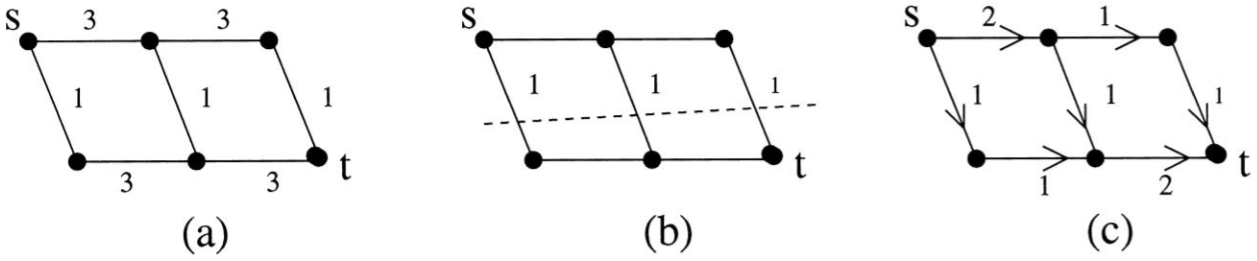
\includegraphics[width=\textwidth]{figs/1-commodity_flow_problem.png}
		\caption{Solution to a 1-commodity flow problem}
		\end{figure}
\end{frame}


\begin{frame}
%\subsection{Multicommodity Flow Problems}
\frametitle{Multicommodity Flow Problems}
\begin{center}
\textit {k $ \ge 1$}\\
\end{center}

$k$ number of commodities, each with source $s_i$, sink $t_i$ and demand $D_i$

\textit{Objective:}\\
simultaneously route $D_i$ units of commodity $i$ from $s_i$ to $t_i$ for each $i$ so that the total amount of all commodities passing through any edge is no greater than its capacity.
%undirected edges the sum of the flow in both directions cannot exceed the capacity of the edge.
%useful to maximize the amount of flow that can be routed for each commodity.
\end{frame}


\begin{frame}
\frametitle{Multicommodity Flow Problems}
\textit{concurrent max-flow:}\\
maximize a common fraction $f$ of each commodity that is routed. In other words the maximum value of $f$ such that $fD_i$ units of commodity $i$ can be simultaneously routed for each $i$ without violating any capacity constraints.

\textit{fairness property:}\\
ensures that proportionally more of one commodity will not be routed at the expense of another.

\textit{min-cut (a.k.a sparset cut $\mathscr{S}$):}\\
the minimum over all cuts of the ratio of the capacity of the cut to the demand of the cut.
\end{frame}

\begin{frame}
\frametitle{Multicommodity Flow Problems}
$$ \mathscr{S} = \underset{U \subseteq V }{min} \frac{C(U,\bar{U})}{D(U,\bar{U})}, $$
where 
$$ C(U,\bar{U}) = \sum_{e \in \langle U, \bar{U} \rangle} C(e) $$
is the sum of capacities of the edges linking $U$ to $\bar{U}$ and 
$$ D(U,\bar{U}) = \sum_{ \{ i | s_i \in U \land t_i \in \bar{U}\quad or \quad t_i \in U \land s_i \in \bar{U} \} } D_i $$
is the sum of the demands whose source and sink are on opposite sides of the cut that separates $U$ from $\bar{U}$
\end{frame}

\begin{frame}[c]
\frametitle{Multicommodity Flow Problems}
	\begin{figure}
		\centering
		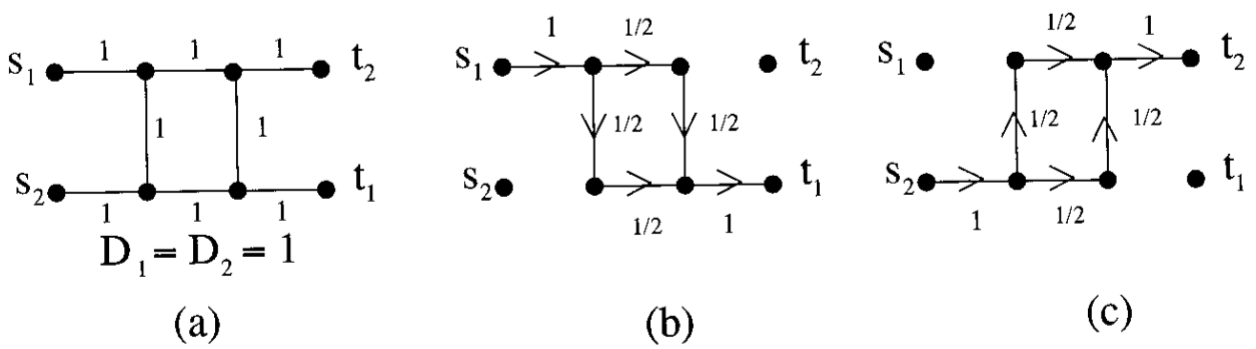
\includegraphics[width=\textwidth]{figs/2-commodity_flow_problem.png}
		\caption{Solution to a 2-commodity flow problem}
	\end{figure}
\end{frame}


\begin{frame}
\frametitle{Multicommodity Flow Problems}
Check that the \textit{max-flow} is always upper bounded by the \textit{min-cut} for any multicommodity flow problem. Let $i_1,i_2,i_3,\dots,i_r$ denote the commodities  whose source and sink are separated by some cut $\langle U, \bar{U} \rangle$
$$	\sum_{j=1}^{r} fD_{i_{j}} \le C(U, \bar{U})	$$
Since
$$	\sum_{j=1}^{r} D_{i_{j}} = D(U, \bar{U})	$$
this means that
$$	f \le \frac{C(U, \bar{U})}{D(U, \bar{U})}	$$
%the max flow is upper bounded by the min-cut
\end{frame}


\begin{frame}
%\subsection{Prior work on max-flows and min-cuts for multicommodity flow problems}
\frametitle{Prior work on max-flows and min-cuts for multicommodity flow problems}
Schrijver [1990]\\
If the graph formed by the set of demands does not contain either three disjoint edges or a triangle and a disjoint edge\\
\quad ---> \quad \textit{max-flow and min-cut are equal}

Example: when there is a commodity for every pair of nodes and all demands are equal, the max-flow and min-cut are equal provided that the dual of the flow problem satisfies a certain cut condition.

\textit{general networks}\\  
The max-flow is within a factor of $k$ of the min-cut since each commodity can be optimized separately using 1/k of the capacity of each edge.
\end{frame}

\begin{frame}
\frametitle{Prior work on max-flows and min-cuts for multicommodity flow problems}
	\begin{figure}
 		\centering
    		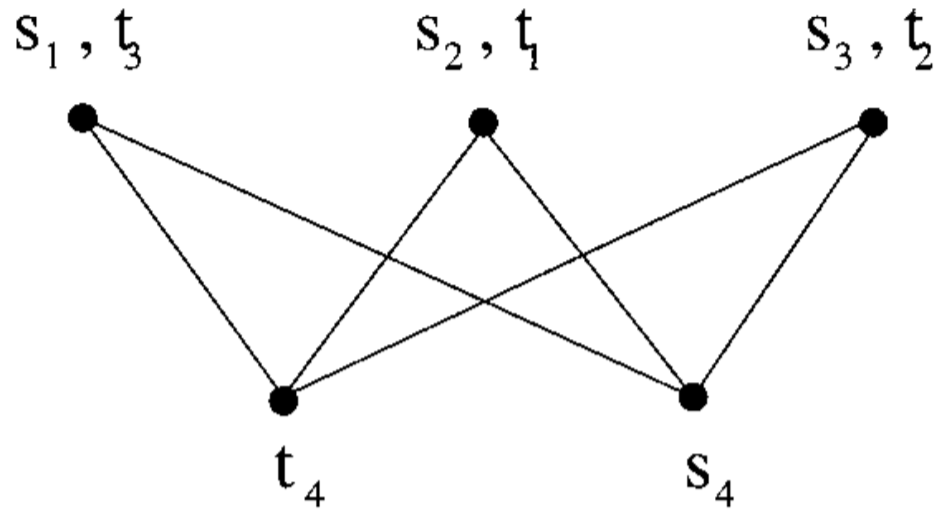
\includegraphics[width=0.5\textwidth]{figs/3-Okamura_Seymour.png}
		\caption{Okamura-Seymour [1981] with max-flow=3/4 and min-cut=1}
	\end{figure}
\end{frame}


\begin{frame}
%\subsection{Max-flow min-cut results}
\frametitle{Max-flow min-cut results}
	 \textit{UMFP (Uniform Multicommodity Flow Problem)}\\
	 In this kind of flow problem there is a commodity for every pair of nodes and the demand for every commodity is the same. WLOG the demand for every commodity is set to one.
	 %Without Loss Of Generality
\end{frame}

\begin{frame}
\frametitle{Max-flow min-cut results}
\begin{block}{What is going to be proved?}
	\begin{itemize}
		\item An approximate max-flow min-cut theorem for uniform multicommodity flow problems. 
		The max flow is within a $\Theta (\texttt{log} n)$-factor of the min-cut. 
		\item The previous bound is tight in the sense that there exist uniform flow problems for which the max-flow is precisely a factor of $\Theta(\texttt{log}n)$ smaller than the min-cut for any $n$.
		% Also we show that this bound is tight in the sense that there exist uniform flow problems for which the max-flow is precisely a factor of $\Theta(\texttt{log}n)$ smaller than the min-cut for any $n$.
	 \end{itemize} 
\end{block}
\end{frame}


\begin{frame}
\frametitle{Max-flow min-cut results}
What is $\Theta$?\\
For a given function $g(n)$, we denote by $\Theta (g(n))$ the set of functions
\begin{equation*}	
	\begin{split}
		\Theta(g(n)) = \{ f(n) : & \text{ $\exists \quad c_1, c_2 > 0$ and $n_0$ such that} \\
						 & 0 \le c_1 g(n) \le f(n) \le c_2 g(n) \quad \forall n \ge n_0 \}
	\end {split}
\end{equation*}
\end{frame}

\begin{frame}
\frametitle{Max-flow min-cut results}
	\begin{figure}
 		\centering
    		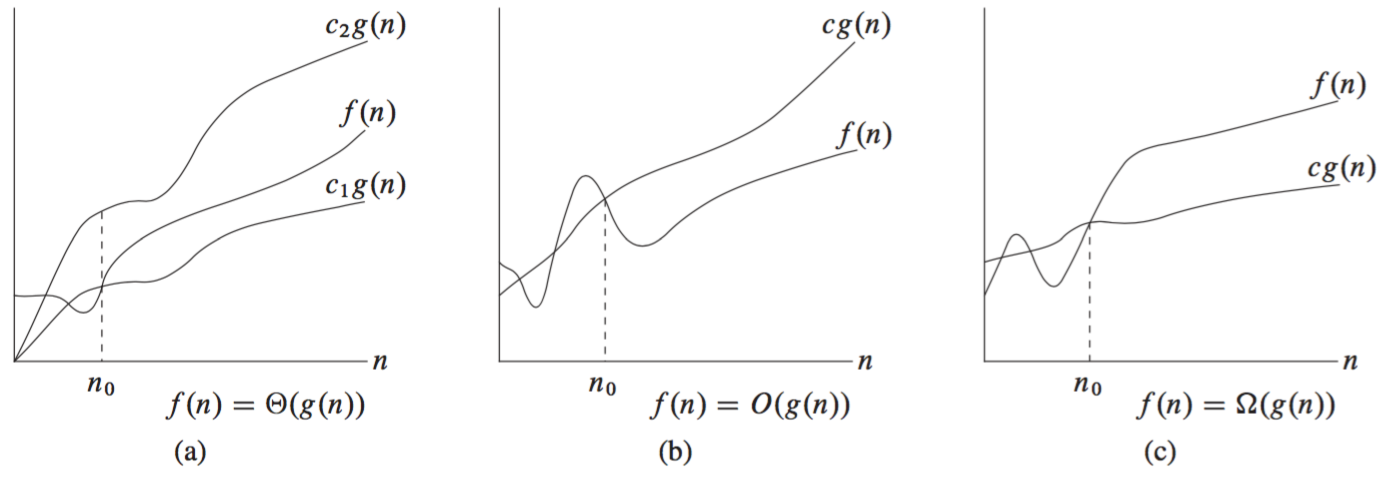
\includegraphics[width=\textwidth]{figs/4-Asymptotic_notation.png}
		\caption{Graphic examples of the $\Theta$, $O$, and $\Omega$  notations. (a) $\Theta$-notation bounds a function to within constant factors. (b) $O$-notation gives an upper bound for a function to within a constant factor. (c) $\Omega$-notation gives a lower bound for a function to within a constant factor.}
%Graphic examples of the $\Theta$, $O$, and $\Omega$  notations. In each part, the value of $n_0$ shown is the minimum possible value; any greater value would also work. (a) $\Theta$-notation bounds a function to within constant factors. We write $f(n) = \Theta (g(n))$ if there exist positive constants $n_0$, $c_1$, and $c_2$ such that at and to the right of $n_0$, the value of $f(n)$ always lies between $c_1 g(n)$ and $c_2 g(n)$ inclusive. (b) $O$-notation gives an upper bound for a function to within a constant factor. We write $f(n) = O(g(n))$ if there are positive constants $n_0$ and $c$ such that at and to the right of $n_0$, the value of $f(n)$ always lies on or below $cg(n)$. (c) $\Omega$-notation gives a lower bound for a function to within a constant factor. We write $f(n) = \Omega (g(n))$ if there are positive constants $n_0$ and $c$ such that at and to the right of $n_0$, the value of $f(n)$ always lies on or above $cg(n)$.
	\end{figure}
\end{frame}



\begin{frame}
%\subsection{Applications to Approximation Algorithms}
\frametitle{Applications to Approximation Algorithms}
In a UMFP we have:\\
\textit{Demand} across a cut $\langle U, \bar{U} \rangle$ 
%is the product of the number of nodes in $U$ and the number of nodes in $\bar{U}$
$$D(U,\bar{U}) = |U||\bar{U}|$$
\textit{Min-cut} of uniform flow problem is
$$ \mathscr{S} = \underset{U \subseteq V}{min} \frac{C(U,\bar{U})}{ |U||\bar{U}|}$$
where $C(U,\bar{U}) = \sum_{e \in \langle U, \bar{U} \rangle } C(e)$.\\
In the case when all capacities are 1, the min-cut is simply
$$ \mathscr{S} = \underset{U \subseteq V}{min} \frac{| \langle U,\bar{U}\rangle |}{ |U||\bar{U}|}$$
\end{frame}

\begin{frame}
\frametitle{Applications to Approximation Algorithms}
\textit{min-cut} is a good measure of the number of edges that need to be removed in order to partition the underlying network into pieces of various sizes.

\textit{Consequence:} able to use our algorithm for finding an approximate min-cut to design the first nontrivial polynomial-time approximation algorithms for several important NP-hard graph partitioning problems.
\end{frame}


\begin{frame}
%\subsection{Subsequent Work}
\frametitle{Subsequent Work}
More literature and results of this paper was published at the first time in an extended abstract of Leighton and Rao [1988].\\

Subsequent work:
\begin{itemize}
	\item Klein et al. [1995] the max-flow is always within an $O(\texttt{log} C \texttt{log} D)$ factor of the min-cut for undirected multicommodity flow problems.
	\item Tragoudas [1990], Plotkin and Tardos [1993] and Garg et al. [1996] have improved the previous bound to $O(\texttt{log}^2 k)$
	\item Linial  et al. [1995] and Aumann and Rabani [1998] established an existentially tight gap of $\Theta(\texttt{log} k)$ with the use of Bourgain's technique with embed spaces on graphs into geometric spaces.
\end{itemize}
\end{frame}	

\begin{frame}
\frametitle{Subsequent Work}
\begin{itemize}	
	\item Garg  et al. [1996] established an $O(\texttt{log} k)$  max-flow min-cut theorem for arbitrary (undirected) multicommodity flow problems where the sum of the flows is maximized. 
	\item Klein et al. [1993] discovered a $\Theta(1)$ max-flow min-cut theorem for uniform multicommodity flow problems in undirected planar graphs and graphs with small excluded minors.
	\item Klein et al. [1997] and Even et al. [1998] $O(\texttt{log}^3 k)$ max-flow min-cut theorem for multicommodity flow problems in directed networks for which the demand from any node u to any node v is equal to the demand from v to u. 
\end{itemize}
\end{frame}





%!TEX root = presentazioneNBD.tex

\setlength{\parskip}{\baselineskip} 
\section{Max-Flow Min-Cut Theorems}
\begin{frame}[t]
\frametitle{Max-Flow Min-Cut Theorems}
\begin{block}{What is going to be proved?}
	\begin{itemize}
		\item Uniform Multicommodity Flow Problem 
        \begin{itemize}
			\item Worst case: The Max-Flow is a $\Omega(\log n)$-factor smaller than the min-cut
            \item Finding Small Cuts in UMFPs: The Max-Flow is always within a $\Theta(\log n)$-factor of the min-cut for any UMFP
		\end{itemize}
	 	\item Product Multicommodity Flow Problem
        \begin{itemize}
			\item The Max-Flow is within a $\Theta(\log n)$-factor of the min-cut for any PMFP
		\end{itemize}
	 \end{itemize} 
\end{block}
\end{frame}

\begin{frame}
\frametitle{Uniform Multicommodity Flow Problem: Worst case}
Consider the network G with the following properties:
\begin{itemize}
	\item 3- \emph{regular} graph,
	\item \emph{n} nodes,
	\item \emph{unit} edge capacity,
    \item  $| \left \langle U, \bar{U} \right \rangle | \geq c \quad min \{| U | ,  | \bar{U}  | \}$ where $c>0$ and $U\subseteq V$.
\end{itemize}

The Min-Cut of the corresponding UMFP is 

$$\mathscr{S} = \underset{U\subseteq V}{min} \frac{\left | \left \langle U, \bar{U} \right \rangle \right |}{\left | U \right |\left | \bar{U} \right |} \geq \underset{U\subseteq V}{min} \frac{c}{max \left \{ \left | U \right |, \left | \bar{U} \right | \right \}} = \frac{c}{n-1}$$
\end{frame}

\begin{frame}
\frametitle{Uniform Multicommodity Flow Problem: Worst case}

We proceed computing the max-flow in order to verify how far it is from the min-cut.

Since the graph is 3-regular, at most $\frac{n}{2}$ of the nodes are within distance $\log n -3$ of any particular node $v \in V$.

Hence, for at least half of the $\binom{n}{2}$ commodities, the length of the \emph{shortest path} that connects the \emph{source} to the \emph{sink} in \emph{G} is at least $\log n -2$ edges.

Thus, to allow a flow of \emph{f}, for such a commodity, at least $f(\log n -2)$ capacity must be used.

\end{frame}

\begin{frame}
\frametitle{Uniform Multicommodity Flow Problem: Worst case}

So, to sustain a flow \emph{f} for all the $\binom{n}{2}$ commodity, the capacity of the network must be at least
$$\frac{1}{2}\binom{n}{2}f(\log n - 2)$$

Due to the \emph{unit} capacity edges, the total capacity is at most $\frac{3n}{2}$. So that for the \emph{capacity constraint},

$$f\leq \frac{3n}{\binom{n}{2}(\log n - 2)} = \frac{6}{(n-1)(\log n -2)}\leq \frac{6\mathscr{S}}{c(\log n -2)}= O\left ( \frac{\mathscr{S}}{\log n} \right )$$

Thus, the max-flow for the UMFP on \emph{G} is at least $\Theta(\log n)$.

\end{frame}

\begin{frame}
\frametitle{Uniform Multicommodity Flow Problem: Worst case}

The following theorem summarizes what has been shown above.

\emph{For any n, there is an n-node uniform multicommodity flow problem with max-flow f and min-cut $\mathscr{S}$ for which} $f \leq O\left ( \frac{\mathscr{S}}{\log n} \right )$.

\end{frame}

\begin{frame}
%\frametitle{Uniform Multicommodity Flow Problem: Finding Small Cuts in UMFPs}

%We are now going to prove using two different algorithms that the case analyzed previously is the worst one in the sense that the min-cut of a UMFP can never be more than $\Theta(\log n)$.
%\begin{block}{Algorithms for finding a small cut in UMFPs}
%	\begin{itemize}
%		\item Polynomial-time algorithm     
%	 	\item Algorithm that tends to place in the cut edges with large distance
        
%	 \end{itemize} 
%\end{block}

%\end{frame}

%\begin{frame}
\frametitle{Uniform Multicommodity Flow Problem: Finding Small Cuts in UMFPs}

There is a polynomial-time algorithm that finds a cut $\left \langle U, \bar{U} \right \rangle$ for any UMFP for which 
$$\frac{C(U,\bar{U})}{|U||\bar{U}|} \leq O(f \log n)$$  

The quantity $\frac{C(U,\bar{U})}{|U||\bar{U}|}$ is the \emph{ratio cost} of a cut $\left \langle U, \bar{U} \right \rangle$

Recall that the min-cut of a UMFP is 

$$\mathscr{S} = \underset{U\subseteq V}{min} \frac{C(U,\bar{U})}{\left | U \right |\left | \bar{U} \right |}$$.
\end{frame}

\begin{frame}
\frametitle{Uniform Multicommodity Flow Problem: Finding Small Cuts in UMFPs}

\emph{For any uniform multicommodity flow problem,}

$$\Omega\left ( \frac{\mathscr{S}}{\log n} \right ) \leq f \leq \mathscr{S}$$

\emph{where f is the max-flow and $\mathscr{S}$ is the min-cut of the UMFP}.

The algorithm for finding the cut is based on the linear programming dual of the UMFP. 
\end{frame}

\begin{frame}
\frametitle{Uniform Multicommodity Flow Problem: Finding Small Cuts in UMFPs}

%A multicommodity problem for a graph \emph{G} consists in apportioning a fixed amount of weight (thought as distances) to the edges of \emph{G} so as to maximize the comulative distance between the \emph{source/sink} pairs.

The dual of \emph{k}-commodity flow problem consists of finding a nonnegative distance $d(e)$ for each edge $e \in E$ so that

$$\sum_{i=1}^{k}D_i d(s_i,t_i) \geq 1$$

and so that 
$$\sum_{e \in E} C(e)d(e)$$

is minimized, where $d(s_i,t_i)$ is the distance between the \emph{source} and the \emph{sink} for the \emph{i-th} commodity in \emph{G}.
\end{frame}

\begin{frame}
\frametitle{Uniform Multicommodity Flow Problem: Finding Small Cuts in UMFPs}

In the case of uniform multicommodity flow the distance constraint is
$$\sum_{u,v \in V}d(u,v) \geq 1$$

Then, we define 

$$W = \sum_{e \in E} C(e)d(e)$$

as the \emph{total weight} of the distance function.
\end{frame}

\begin{frame}
\frametitle{Uniform Multicommodity Flow Problem: Finding Small Cuts in UMFPs}

By solving the dual problem we can find a distance $d(e)$ that satisfies the distance constraint and for which $W=f$.

We are now going to explore another way to find a good cut with ratio cost at most $O(W\log n) = O(f\log n)$.
\end{frame}


\begin{frame}
\frametitle{Uniform Multicommodity Flow Problem: Alternative way to find the cut}

For this purpose we refer to the following lemma:

\emph{For any graph G with arbitrary edge capacities, any} $\Delta>0$, \emph{and any distance function with total weight W it is possible to partition G into components with radius at most} $\Delta$ \emph{so that the capacity of the edges connecting nodes in different components is at most} $\frac{4W\log n}{\Delta}$

\end{frame}

\begin{frame}
\frametitle{Uniform Multicommodity Flow Problem: Proof lemma}

Let $C = \sum_{e \in E} C(e)$ be the total capacity on the edges of \emph{G}

\begin{itemize}
\item When $\Delta \leq \frac{4W\log n}{C}$ we use the partition where each node is in a different component. Each component has radius $\Delta \geq 0$ and the capacity of the edges running between the components is at most $\frac{4W\log n}{\Delta}$.

\item When $\Delta \geq \frac{4W\log n}{C}$ we proceed with the construction of a second graph $G^{+}$
\end{itemize}

\end{frame}

\begin{frame}
\frametitle{Uniform Multicommodity Flow Problem: Build $G^{+}$}

\begin{itemize}
\item Replace each edge of \emph{G} with a path of $\left \lceil \frac{Cd(e)}{W} \right \rceil$ edges
\item Assign to each edge of the path capacity $C(e)$ and distance 1
\end{itemize}

Thus, create the partitions

\begin{itemize}
\item Select an arbitrary node $v \in G^{+}$ that corresponds to a node in G
\item For each $i \geq 0$ define $G_i^{+}$ to be the subgraph of $G^{+}$ consisting of nodes and edges within distance $i$ of $v$
\end{itemize}
\end{frame}

\begin{frame}
\frametitle{Uniform Multicommodity Flow Problem: Partition $G^{+}$}

Let 
\begin{itemize}
\item $C_0 = \left ( \frac{2C}{n} \right )$ for $i>0$
\item $C_i$ the total capacity of the edges in $G_{i}^{+}$
\end{itemize}

Denoting with $j$ the smallest value of $i\geq 0$ for which $C_{i+1} < (1+\epsilon)C_i$, where $\epsilon = \frac{W \log n}{\Delta C}<\frac{1}{4}$.

The nodes and edges in $G_j^{+}$ form the first component of the partition. The other components are built by removing $G_j^{+}$ from $G^{+}$ and then repeat the entire process until there are no longer nodes $v \in G^{+}$ that correspond to nodes in $G$.

\end{frame}

\begin{frame}
\frametitle{Uniform Multicommodity Flow Problem: Proof}

Define $C^{+}$ the total initial capacity of $G^{+}$. Depending on the construction of $G^{+}$ we know that 

$$C^{+} = \sum_{e \in E} C(e)\left \lceil \frac{Cd(e)}{W} \right \rceil \leq \sum_{e \in E}C(e) + \frac{C}{W}\sum_{e \in E}C(e)d(e) = 2C$$

Since the $G^{+}$ partitions of $G^{+}$ are disjoint, the total capacity on all edges leaving all components in $G^{+}$ is at most

$$\epsilon(C^{+}+nC_0) \leq 2\epsilon C^{+} 2\epsilon C = 4\epsilon C$$
\end{frame}

\begin{frame}
\frametitle{Uniform Multicommodity Flow Problem: Proof}

The partition for $G$ is derived from the components of $G^{+}$. Two nodes of $G$ are in the same partition of $G \Leftrightarrow$ are in the same component in $G^{+}$.

Moreover, any $e \in G$ that links two components in $G$ corresponds to a path of capacity $C(e)$ edges in $G^{+}$ that was cut to form at least one of the corresponding components in $G^{+}$.

So that, the total capacity of the edges linking different components in $G$ is at most $4\epsilon C = \frac{4W\log n }{\Delta}$.

\end{frame}

\begin{frame}
\frametitle{Uniform Multicommodity Flow Problem: Ratio cost}

Recall that we want to check that the value that the ratio cost of a cut is at most $O(W\log n)$, we proceed with the following

\emph{For any graph G and any distance function with total weight W, we can either
\begin{itemize}
\item find a component with radius $\frac{1}{2n^2}$ that contains at least $\frac{2}{3}$ of the nodes in G
\item find a cut of G with ratio cost $O(W\log n)$
\end{itemize}}
\end{frame}

\begin{frame}
\frametitle{Uniform Multicommodity Flow Problem: Ratio cost}

Apply the result of the previous lemma using $\Delta = \frac{1}{2n^2}$

\begin{itemize}
\item Whether one of the components obtained applying the lemma contains at least $\frac{2}{3}$ of the nodes of $G$ we are done
\item Otherwise we divide the components into two sets so that each sets contains at least $\frac{n}{3}$ nodes $\rightarrow$ the edge capacity of the cut is at most $\frac{4W\log n}{\Delta} = 8Wn^2 \log n$
$$\Downarrow$$
$$\frac{8Wn^2 \log n}{\left ( \frac{2n}{3} \right )\left ( \frac{n}{3} \right )} = 36W\log n = O(W \log n)$$
\end{itemize}
\end{frame}

\begin{frame}
\frametitle{Uniform Multicommodity Flow Problem: Further theorems}

\begin{itemize}
\item \emph{For any graph $G$, if there is a distance function $d$ with total weight W and a subset of nodes $T \subseteq V$ with $|T|\geq \frac{2n}{3}$ and $\sum_{u \in V-T}d(T,t) \geq \frac{1}{2n}$ then we can find a cut with ratio cost $O(W)$} 
\item \emph{Given a graph $G$ and a distance function with total weight W that satisfies the distance contraint, we can find a cut with ratio cost $O(W\log n)$}
\end{itemize}
\end{frame}

\begin{frame}
\frametitle{Product Multicommodity Flow Problem}

In a PMFP 
\begin{itemize}
\item Each node $u \in V$ is associated with a nonnegative weight $\pi (u)$
\item The demand for the commodity between nodes $u$ and $v$ is set to be $\pi (u) \pi (v)$
\end{itemize}

In what follows, we will show how to find a cut $\left \langle U, \bar{U} \right \rangle$ for which the weighted ratio cost

$$\frac{C(U,\bar{U})}{\pi (U)\pi (V)}$$

is at most $O(f\log p)$ where $f$ is the max-flow.
\end{frame}

\begin{frame}
\frametitle{Product Multicommodity Flow Problem}
\begin{itemize}
\item Consider $\mathscr{P}$ as the subset of nodes for which $\pi$ is nonzero, and we set $p=|\mathscr{P}|$
\item Assume $\sum_{u \in V}\pi (u) = p$ for each PMFP
\item The number of commodities with nonzero demand is $k = \binom{n}{2}$
\end{itemize}
\end{frame}

\begin{frame}
\frametitle{Product Multicommodity Flow Problem: Theorem}
\emph{For any product multicommodity flow problem with k commodities, 
$$\Omega\left ( \frac{\mathscr{S}}{\log k} \right ) \leq f \leq \mathscr{S}$$
where $f$ is the max-flow and $\mathscr{S}$ is the min-cut of the PMFP.}

Also in that case the cut with small weighted ratio cost is find out with the same algorithm used before, even if in that case the constraint is the following

$$\sum_{\{u,v\} \in \mathscr{P}^2} \pi (u) \pi (v) d(u,v) \geq 1$$

Thus here follow some theorems that are proved using the same procedures just changing some details.
\end{frame}

\begin{frame}
\frametitle{Product Multicommodity Flow Problem: Theorem}

\begin{itemize}
\item \emph{For any graph G, any $\Delta \geq 0$, any distance function with total weight W, and any set of $p$ nodes $\mathscr{P}$ with nonzero node weight, it is possible to partition G into components so that
\begin{itemize}
\item any component containing a node of $\mathscr{P}$ has radius at most $\Delta$
\item the capacity of the edges linking nodes in different components is at most $\frac{4W \log p}{\Delta}$
\end{itemize}}
\item \emph{For any graph G, any distance function with total weight W, and any set $\mathscr{P}$ of $p$ nodes with nonzero node weight, we can either
\begin{itemize}
\item find a component T with radius $\frac{1}{2p^2}$ for which $\pi (T) \geq \frac{2p}{3}$ or
\item find a cut of $G$ with the weighted ratio cost $O(W \log p)$
\end{itemize}}
\end{itemize}
\end{frame}

\begin{frame}
\frametitle{Product Multicommodity Flow Problem: Theorem}

\begin{itemize}
\item \emph{For any node-weighted graph $G$, if there is a distance function $d$ with total weight W and a subset of nodes $T \subseteq V$ for which $\pi (T) \geq \frac{2p}{3}$ and $\sum_{u} \in \mathscr{P}-T \pi (u)d(T,u) \geq \frac{1}{2p}$, than we can find a cut with ration cost $O(W)$}
\item \emph{Given a node-weighted graph G and a distance function with total weight W that satisfies the (weighted) distance-constraint, we can find a cut with weighted ratio cost $O(W \log p)$}
\end{itemize}

\end{frame}
%!TEX root = presentazioneNBD.tex

\setlength{\parskip}{\baselineskip} 
\section{Applications}
\begin{frame}[t]
\begin{block}{Applications to Approximations Algorithms}
	\begin{itemize}
			\item Sparsest Cuts
            \item Flux, Expansion, and Minimum quotient separators
            \item Node cuts
			\item Minimum feedback arc set
            \item Geometric embeddings
        	\item Search Number
            \item Resistance, Conductance, and Rapidly-Mixing Markov Chains
	 \end{itemize} 
\end{block}
\end{frame}


%Networks
\begin{frame}
\frametitle{Introduction to applications}
Max-flow min-cut theorems can be applied to develop good approximation algorithms for a surprisingly wide variety of \textbf{NP-hard} problems. 

Graph partitioning is a critical component of many \textbf{"Dividi et Impera"} [\textit{Philip II of Macedon}] algorithms in practice. 

Unfortunately nearly every variation of the problem is NP-hard and little in the way of approximation algorithms has previously been discovered. 

\end{frame}


%Sparsest Cut
\begin{frame}[t]
\begin{block}{Applications to Approximations Algorithms}
	\begin{itemize}
			\item \textbf{Sparsest Cuts}
            \item Flux, Expansion, and Minimum quotient separators
            \item Node cuts
			\item Minimum feedback arc set
            \item Geometric embeddings
        	\item Search Number
            \item Resistance, Conductance, and Rapidly-Mixing Markov Chains
	 \end{itemize} 
\end{block}
\end{frame}

\begin{frame}
\frametitle{Sparsest Cut}
The sparsest cut of a graph $G=(V,E)$ is a partition $\left \langle U, \bar{U} \right \rangle$ for which:
$$\frac{\left | \left \langle U, \bar{U} \right \rangle \right |}{\left | U \right |\left | \bar{U} \right |}$$

is minimized, where $\left | \left \langle U, \bar{U} \right \rangle \right |$ denotes the number of edges connecting $U$ to $V-U$
\end{frame}

\begin{frame}
\centering
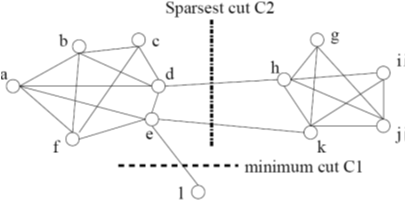
\includegraphics[width=\textwidth]{figs/sparsest_cut.png}
\end{frame}

\begin{frame}
Computing the sparsest cut of a graph is NP-hard .

The sparsest cut can be approximated to within an O(log n) factor using the SMALL CUT (UMFP) algorithm. 

In it's most general form, we desire to find  partition $\left \langle U, \bar{U} \right \rangle$ that minimize:

$$\frac{C(U,\bar{U})}{ \pi(U)\pi(\bar{U}) }$$

The sparsest cut can be approximated to within a factor of O(log p) using the PMFP methods. In this case, we set the capacity of an edge to equal its weight and $\pi(v)$ to be the node weight of v for all  V. 
\end{frame}

%FLUX

\begin{frame}[t]
\begin{block}{Applications to Approximations Algorithms}
	\begin{itemize}
			\item Sparsest Cuts
            \item \textbf{Flux, Expansion, and Minimum quotient separators}
            \item Node cuts
			\item Minimum feedback arc set
            \item Geometric embeddings
        	\item Search Number
            \item Resistance, Conductance, and Rapidly-Mixing Markov Chains
	 \end{itemize} 
\end{block}
\end{frame}

\begin{frame}
A graph has a flux at least $\alpha$if every subset U with at most half of the nodes is connected to the rest of the graph with edges of total weight at least a|U|. 
$$\alpha = \underset{U\subseteq V}{min} \frac{C( U, \bar{U})}{min(\left | U \right |,\left | \bar{U} \right |)} $$
A cut that achieves the flux is called the minimum quotient separator and is related by a constant factor to the sparsest cut since  
$$ \frac{n}{2} \mathscr{S} \le \alpha \le n \mathscr{S}$$
Computing the minimum quotient separator is NP-hard. The sparsest cut algorithms mentioned before provide O(log n).

\end{frame}


%Node Cuts

\begin{frame}[t]
\begin{block}{Applications to Approximations Algorithms}
	\begin{itemize}
			\item Sparsest Cuts
            \item Flux, Expansion, and Minimum quotient separators
            \item \textbf{Node cuts}
			\item Minimum feedback arc set
            \item Geometric embeddings
        	\item Search Number
            \item Resistance, Conductance, and Rapidly-Mixing Markov Chains
	 \end{itemize} 
\end{block}
\end{frame}

\begin{frame}
\frametitle{Node Cut}
Thus far, we have focused our attention on edge cuts for graphs.

These same methods can also be used to derive approximation algorithms for node cuts by converting the node-cut problem for an \textbf{undirected graph} into an edge-cut problem for a \textbf{directed graph}.

A node cut is a \textit{subset of nodes} whose removal from the graph separates the remaining nodes into two disconnected pieces.
\end{frame}

\begin{frame}

\centering
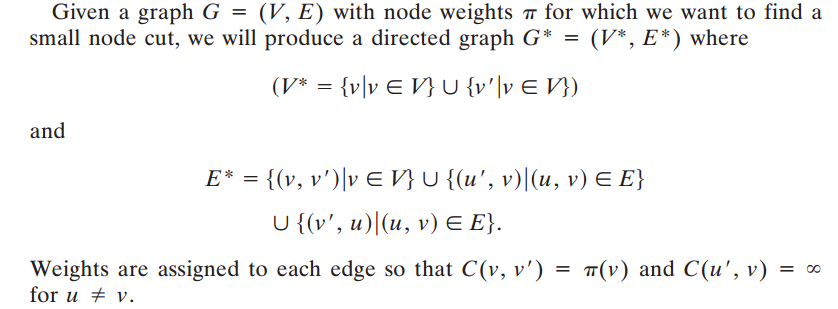
\includegraphics[width=\textwidth]{figs/node_cut.png}
\end{frame}

\begin{frame}
Any node cut in G corresponds to a directed edge cut in G* with the same cost and balance. 
 
The correspondence is as follows: Let U denote the set of nodes that cuts V - U into V1 and V2. 
 Then, the cut of $G^*$ is $\left \langle V^*_1, V^*_2 \right \rangle$  where $V^*_1=\left \{v|v \in V_1 \bigcup U\right \} \bigcup \left \{v'|v \in U \right \}$.
 
 And any directed edge cut in $G^*$ with noninfinite cost corresponds to a node cut in G with the same cost and balance. 
\end{frame}


%Minimum FeedBack arc set
\begin{frame}[t]
\begin{block}{Applications to Approximations Algorithms}
	\begin{itemize}
			\item Sparsest Cuts
            \item Flux, Expansion, and Minimum quotient separators
            \item Node cuts
			\item \textbf{Minimum feedback arc set}
            \item Geometric embeddings
        	\item Search Number
            \item Resistance, Conductance, and Rapidly-Mixing Markov Chains
	 \end{itemize} 
\end{block}
\end{frame}

\begin{frame}
\frametitle{Minimum FeedBack arc set}
The minimum feedback arc set problem
consists of removing the smallest number of edges F from a digraph G so that
the residual graph is \textbf{acyclic}. 

The problem is NP-hard and arises in numerous
applications.
An equivalent formulation of the problem is to find an ordering v1, v2, . . . , vn
of the nodes of G so that the number of forward edges F (i.e., edges of the form
(vi, vj) where i < j) is minimized. 
\end{frame}

\begin{frame}
In order to show that this algorithm produces an ordering with O(F log2n) forward edges where F is the optimal value for the graph, we again
examine the decomposition tree of subgraphs produced by the algorithm. In
particular, let $G_{i,j}$ denote the jth subgraph on level i of the decomposition tree,
and let $S_{i,j}$ denote the optimal directed bisection for $G_{i,j}$. 

Then the number of forward edges for the ordering produced by the algorithm is
\end{frame}

\begin{frame}
\centering
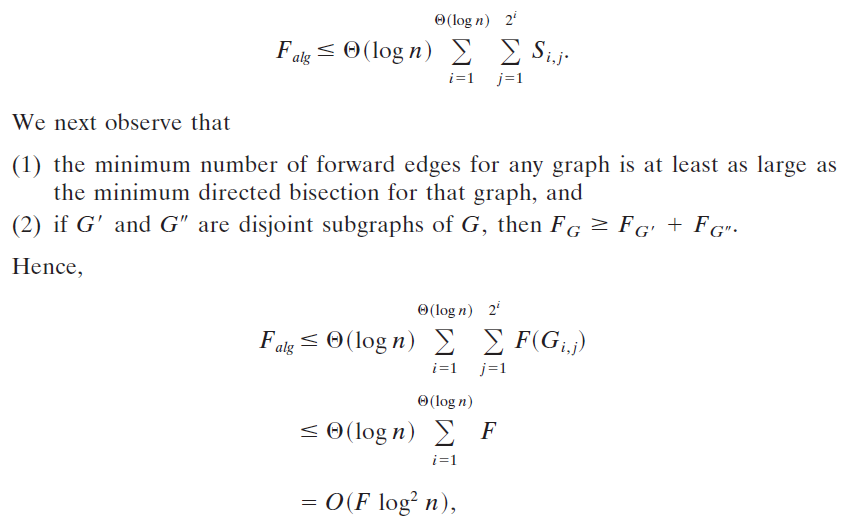
\includegraphics[width=\textwidth]{figs/Feedback_arc_set.png}
\end{frame}


%Geometric Embeddings
\begin{frame}[t]
\begin{block}{Applications to Approximations Algorithms}
	\begin{itemize}
			\item Sparsest Cuts
            \item Flux, Expansion, and Minimum quotient separators
            \item Node cuts
			\item Minimum feedback arc set
            \item \textbf{Geometric embeddings}
        	\item Search Number
            \item Resistance, Conductance, and Rapidly-Mixing Markov Chains
	 \end{itemize} 
\end{block}
\end{frame}


\begin{frame}
\frametitle{GEOMETRIC EMBEDDINGS}
The geometric embedding problem consists of
an edge-weighted graph $G=(V, E)$ and a set of points P in a d-dimensional
Euclidean space. 
The goal is to find an injection $f: V \rightarrow P$ that minimizes the
total edge length D induced on P, where
$$D =\sum_{
(u,v)\in E}
d(f(u), f(v))w(u,v)$$
d( x, y) is the Euclidean distance between points x and y, and w(u, v) is the
weight of edge (u, v). 
\end{frame}

\begin{frame}
From embedding into grids to embedding into an arbitrary graph H with small congestion and dilation. 
An embedding maps nodes of
G to nodes in H and edges in G to paths in H. 
\begin{itemize}
\item The congestion of the embedding
is the maximum for any edge e of H of the number of paths in the embedding
that contain e.
\item The dilation of an embedding is the maximum number of edges in
any path in the embedding.
\end{itemize}

THEOREM:
\textit{Consider any n-node bounded degree graph G and any 1–1
mapping h of the nodes of G onto the nodes of an n-node bounded degree graph H
with flux $\alpha$. The edges of G can be routed as paths in H with congestion and dilation
O(log n/$\alpha$).}

\end{frame}

%Search Number

\begin{frame}[t]
\begin{block}{Applications to Approximations Algorithms}
	\begin{itemize}
			\item Sparsest Cuts
            \item Flux, Expansion, and Minimum quotient separators
            \item Node cuts
			\item Minimum feedback arc set
            \item Geometric embeddings
        	\item \textbf{Search Number}
            \item Resistance, Conductance, and Rapidly-Mixing Markov Chains
	 \end{itemize} 
\end{block}
\end{frame}

\begin{frame}
\frametitle{ SEARCH NUMBER}
The search number of a graph is the number of searchers needed to capture a fugitive that can move with arbitrary speed about the edges of the graph.

A search step is the placing of
a searcher on a vertex, the movement along an edge, or the removal from a vertex. A search sequence is a sequence of search steps.

An edge e=( x, y) becomes clear when:
\begin{itemize}
\item there is a searcher on x and a second searcher moves from x to y
\item all the edges
other than e incident to x are clear and a searcher moves from x to y. 

A clear edge e can become contaminated again if the movement or removal of a searcher
results in a path from a contaminated edge to e that includes no nodes containing
a searcher.

\end{itemize}
\end{frame}

\begin{frame}
A search strategy for a graph is a search sequence that results in \textbf{
edges being simultaneously clear}. The search number of a graph is the minimum
number of searchers for which a search strategy exists.

Kirousis and Papadimitriou [1986] show that the node search number of a
graph is equal to its pathwidth plus one.  

Our results give an O(log2n)
approximation algorithm for finding the search number and node search number
of a graph.
\end{frame}


%RESISTANCE, CONDUCTANCE, AND RAPIDLY-MIXING MARKOV CHAINS.

\begin{frame}[t]
\begin{block}{Applications to Approximations Algorithms}
	\begin{itemize}
			\item Sparsest Cuts
            \item Flux, Expansion, and Minimum quotient separators
            \item Node cuts
			\item Minimum feedback arc set
            \item Geometric embeddings
        	\item Search Number
            \item \textbf{Resistance, Conductance, and Rapidly-Mixing Markov Chains}
	 \end{itemize} 
\end{block}
\end{frame}

\begin{frame}
\frametitle{RESISTANCE, CONDUCTANCE, AND RAPIDLY-MIXING MARKOV CHAINS.}

Reversible Markov Chains are often identified with a weighted directed graph
$G=(V, E)$ where the weight $\pi(v)$ of a node v is the probability of being in
state v in the stationary distribution and the weight $w(e)$ of an edge $e=(u, v)$ is
$\pi(u)P(u,v)$ where $P(u,v)$ is the probability of moving to state v from state u.
\begin{itemize}
\item The conductance C of the chain is equal to the flux of G and is useful in
quantifying the most severe transition bottleneck in the chain.
\item The resistance R of
the chain is the minimum capacity needed on each edge in order that there exist
a solution to the PMFP where $\pi(u)\pi(v)$ flow is passed between $u$ and $v$ $\forall
v \in V$. 
\end{itemize}
\end{frame}

\begin{frame} 
As a consequence of the inequality:
$$\Omega (\frac{\mathscr{S}}{log k}) \le f \le \mathscr{S}$$ , we can conclude that for any chain, $C^{-1}$ and
$R$ are equal up to a Q(log p) factor, where p is the number of non zero states in the chain.

A Markov chain is said to be rapidly-mixing if the chain reaches equilibrium
quickly. The mixing rate of a chain is often characterized in terms of its second
eigenvalue, which is known to be within a square of the conductance. 
\end{frame}




\setbeamercolor{background canvas}{bg=matblue}
\setbeamercolor{normal text}{fg=white}
\begin{frame}[plain, b]
\centering
\huge \textcolor{white}{Thank You}
\normalsize

\vspace*{\fill}

 \begin{beamercolorbox}[wd=\paperwidth]{section in head/foot}
 \centering
Multicommodity Max-Flow Min-Cut Theorems and Their Use in Designing Approximation Algorithms
\vskip10pt
\end{beamercolorbox}
 \end{frame}

\end{document}
